
\section{Introduction}

Coreset selection is a technique designed to reduce the size of training data while maintaining the performance of predictive models~\citep{guo2022deepcore}.
%
By carefully identifying a representative subset of the original dataset, this approach addresses critical challenges such as computational efficiency and memory limitations.
%
Coresets are constructed to capture the most informative and diverse samples, ensuring that the essential characteristics of the underlying data distribution are preserved.
%
This makes the method especially valuable in scenarios involving large-scale datasets or resource-constrained environments, where processing the entire dataset may be infeasible.
%
Coreset selection finds broad applications in areas such as data summarization, accelerating model training, reducing annotation costs, and improving model interpretability.
%
It is also practically applied to technologies that require retaining useful training instances, such as continual learning and active learning~\citep{sener2017active, toneva2019forgetting, paul2021deep, ducoffe2018adversarial, margatina2021active}.
%
As machine learning advances into more complex domains, coreset selection will become increasingly critical for balancing efficiency and scalability.

This paper addresses the problem of coreset selection in scenarios where the future deployment environment of the model is uncertain.
%
This challenge frequently arises in applications that require models to be tailored to specific, and often unpredictable, conditions or environments.
%
For example, it includes tasks such as assessing investment risks under fluctuating economic conditions, predicting medical outcomes across diverse demographic groups, and estimating agricultural yields under varying climate scenarios.
%
In such settings, the ability to create a representative and compact subset of the data that ensures reliable model performance is crucial.
%
Traditional coreset selection does not make the assumption that future test distributions are uncertain, and it is unclear whether the model will work effectively under such conditions.
%
The objective of this study is to develop a methodology for selecting a coreset from the original dataset while explicitly accounting for the need for worst-case robustness. This enables the model to perform effectively even under uncertain and variable future deployment conditions.

In this study, we focus on a distributionally robust setting under covariate shift conditions, which is a critical challenge in many real-world machine learning applications.
%
Covariate shift occurs when the distribution of input features changes between the training and deployment (test) phases.
%
Distributionally robust learning~\citep{goh2010distributionally, delage2010distributionally, chen2021distributionally} aims to tackle this problem by optimizing model performance under worst-case distributional shifts, enabling models to perform effectively across a wide range of potential data distributions and ensuring robustness to variability and uncertainties.
%
Within this context, we address the specific problem of selecting a robust coreset, assuming that the future covariate distribution may deviate within a defined range from the distribution of the original dataset.
%
To this end, we propose a novel method, termed the \emph{Distributionally Robust Coreset Selection (DRCS)} method, which focuses on constructing a representative and robust subset of data tailored for these challenging conditions.

The basic idea of the DRCS method is to select a coreset that minimizes the worst-case test error under uncertain future test distributions, addressing the challenge of ensuring robustness in the face of potential distributional shifts.
%
To achieve this, we derive a novel and theoretically grounded upper bound for the worst-case test error in the context of distributionally robust covariate shift.
%
This upper bound serves as a critical foundation for guiding the coreset selection process.
%
Building on this theoretical insight, we propose an efficient algorithm designed to select a coreset that approximately minimizes this upper bound, ensuring that the resulting subset of data is both compact and robust to changes in future test distributions.
%
Although the method is primarily developed for problems formulated within a specific class of convex optimization frameworks, it is versatile and can be extended to coreset selection for deep learning models by leveraging the neural tangent kernel (NTK) or fine-tuning scheme.

\begin{figure}[H]
	\centering
	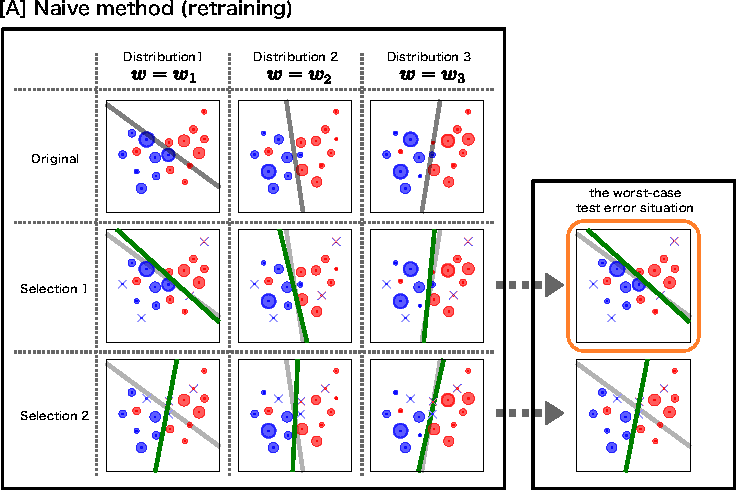
\includegraphics[width=0.8\hsize]{fig/concept1.pdf}
	\caption{
	% この図は、本研究のCoreset selectionのイメージ図である。
	%
	The concept of coreset selection in this study.
	%
	In the left panel, each plot shows the distribution of the training data, where each column represents patterns of distribution changes, while each row represents patterns of instance selection.
	%
	Let gray lines represent the learned results with specified weights and all instances, while green lines the retrained results with specified weights and selected instances.
	%
	The goal is to obtain a selection pattern that can suppress the degradation of test error, even in the worst-case distribution for each selection pattern.
	%
	In this figure, through the three distributions, Selection 1 can be considered a better choice than Selection 2.
	%
	It is practically impossible since we need to explore such worst-case test error for all distributions and selection patterns.
	}
	\label{fig:concept1}
\end{figure}

\begin{figure}[H]
	\centering
	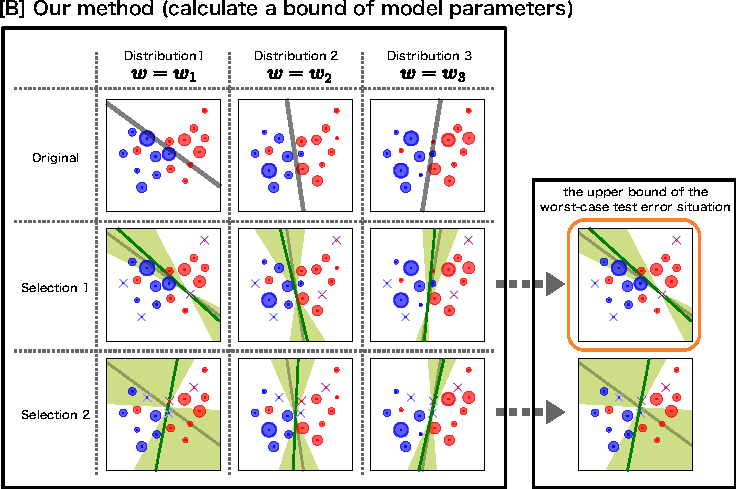
\includegraphics[width=0.8\hsize]{fig/concept2.pdf}
	\caption{
	% この図は、本研究のCoreset selectionのイメージ図である。
	%
	The concept of coreset selection in this study.
	%
	This figures also show the distribution of the training data.
	%
	The green area indicates the bound of model parameters obtained when retraining is performed, and we can analyticaly calculate it before retraining.
	%
	We perform coreset selection to minimize the worst-case test error in the distribution, where the bound becomes the largest among all possible distributions.
	}
	\label{fig:concept2}
\end{figure}

\begin{figure}[H]
	\centering
	\begin{tabular}{cc}
		\begin{minipage}[t]{0.35\hsize}
			\centering
			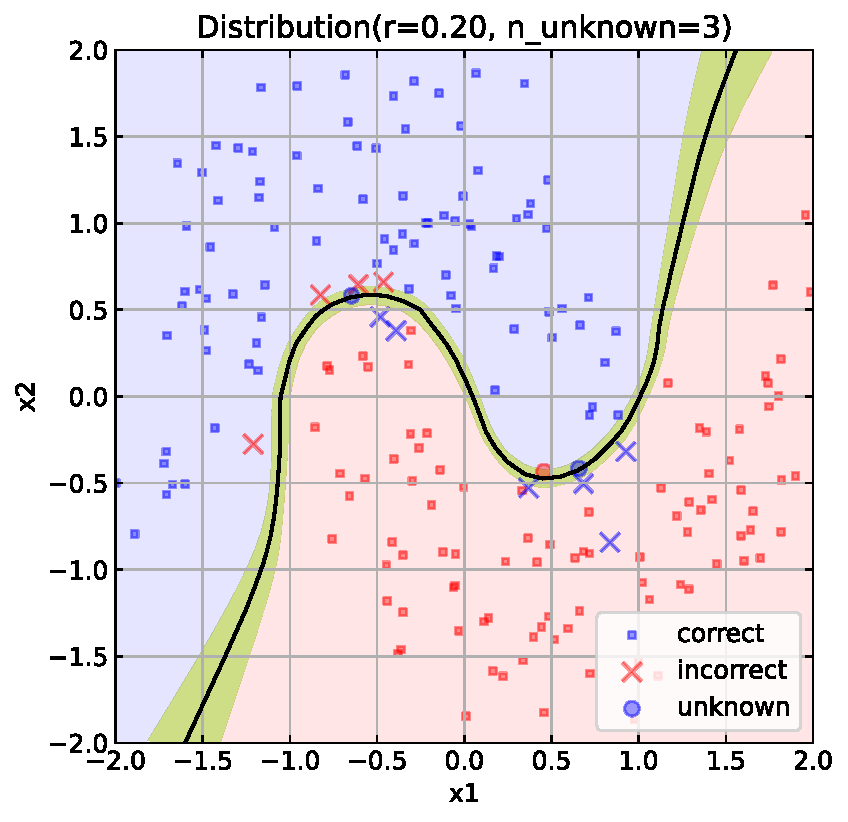
\includegraphics[width=0.95\hsize]{fig/concept3-1.pdf}
			\subcaption{Training instance selection with a reduced bound of model parameters}
			% \subcaption{}
		\end{minipage}
		&
		\begin{minipage}[t]{0.35\hsize}
			\centering
			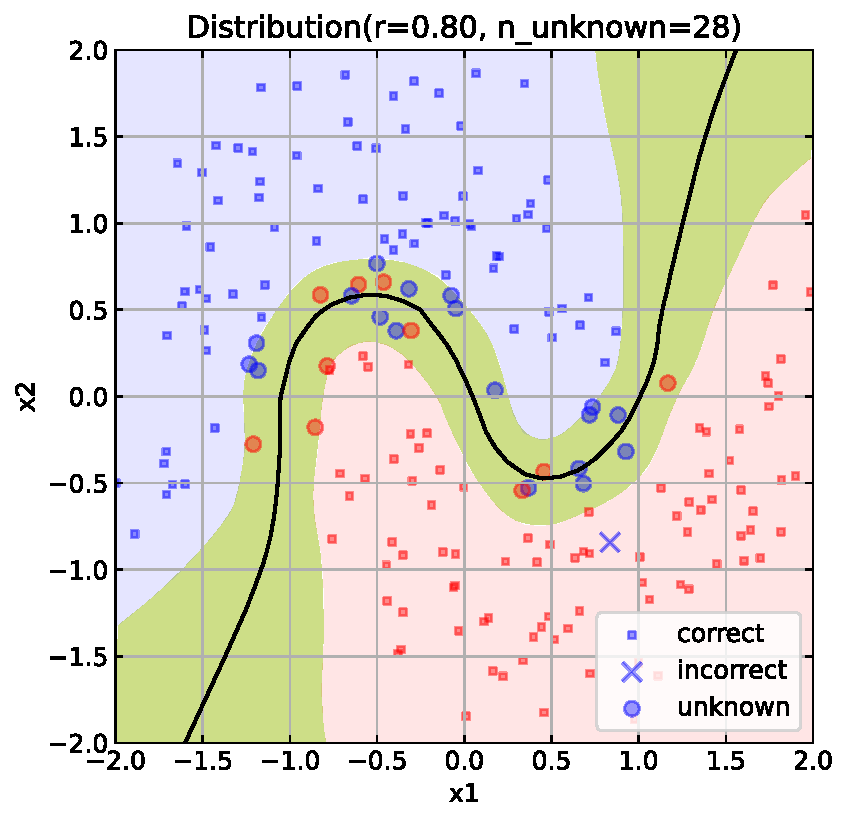
\includegraphics[width=0.95\hsize]{fig/concept3-2.pdf}
			\subcaption{Training instance selection with random sampling}
			% \subcaption{}
		\end{minipage}
		\label{fig:concept2}
	\end{tabular}
	\caption{
		This figure illustrates an upper bound of the validation error in this study.
		%
		Both figures show the distribution of the validation data.
		%
		We calculate a bound of model parameters and use this to derive an upper bound of the validation error.
		%
		In this figure, the blue and red areas represent that the validation data in these areas have a determined classification.
		%
		On the other hand, the validation data in the green area does not have a determined classification.
		%
		As a result, the upper bound of the validation error can be reached in cases where all instances in the green area are incorrectly classified.
		%
		Since the bound of the model parameters depends on how to select instances such as (a) and (b), we perform coreset selection in a distribution where the upper bound of the validation error is minimized.
	}
\end{figure}

\subsection{Contribution}

In this study, we address the challenges discussed in Section~\ref{sec:related-limits} by introducing model parameter bounding techniques.
%
Furthermore, we propose a distributionally robust coreset selection method that provides theoretical guarantees for model performance in binary classification problems.
%
The contributions of this study are as:

\begin{itemize}
	\item We consider the problem of coreset selection under covariate shift environments while taking distributional robustness into account, and propose a method to address this challenge.
	\item In the proposed method, we derive an upper bound of the validation error under the worst-case covariate shift and perform coreset selection to minimize this upper bound.
\end{itemize}